% !TEX root = ../my-thesis.tex
%
\chapter{Resultados}
\label{sec:results}

Los resultados obtenidos de la implementación del problema directo y del problema inverso del EEG, así como el análisis estadístico del estimador, se presentan en tres subsecciones: (i) la solución del problema directo, (ii) la solución del problema inverso, y (iii) el análisis estadístico del error incurrido en el uso de diferentes valores del BSCR en la simulación y posterior localización de fuentes de actividad neuronal. 
A su vez, debido a la gran cantidad de datos obtenidos, se presentan los de mayor relevancia en las figuras y tablas correspondientes, haciendo especial énfasis en los resultados provenientes del uso de los valores de BSCR más referidos en la literatura y los que más se alejan de estos valores, con el fin de comparar los resultados obtenidos y analizar el desempeño del estimador en cada caso.

\section{Solución del Problema Directo}
\label{sec:results:direct}

Las señales de EEG simuladas obtenidas de la implementación del problema directo se muestran en la \cref{fig:eeg-simulated}. 
Estas señales corresponden a BSCR = de 20, 80, 10 y 200, respectivamente, generadas por el dipolo ubicado en la zona somatosensorial y simuladas con un SNR de 1\% proveniente de la fuente.
En cada gráfica, se superponen las señales individuales capturadas por cada uno de los 63 electrodos considerados en el análisis, creando un gráfico de mariposa donde el eje horizontal representa el tiempo y el eje vertical representa la amplitud de la señal. 
Este conjunto de señales son una parte del total de las 9000 señales simuladas por las 100 pruebas de cada permutación de BSCR, SNR y fuente de actividad neuronal.

\begin{figure}[tbp]
    \centering
    \begin{subfigure}{0.9\textwidth}
        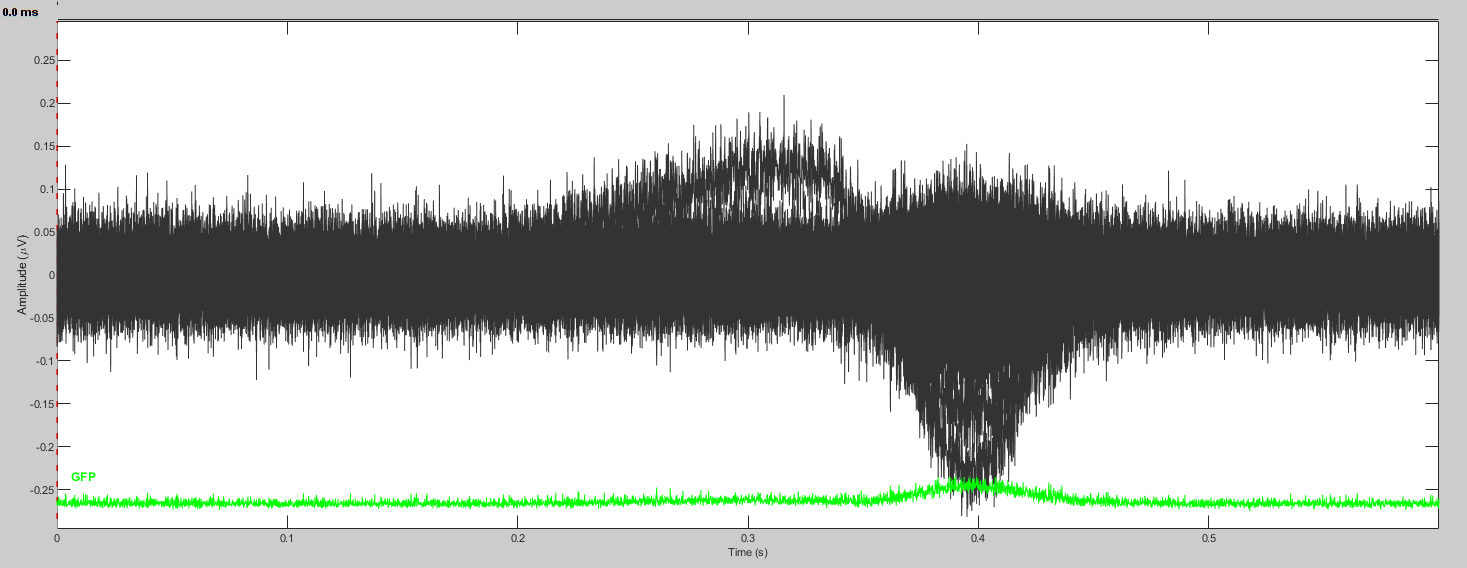
\includegraphics[width=\textwidth]{eeg/eeg-d1n1c8c8.png}
        \caption{Señales de EEG simuladas con BSCR = 10.}
        \label{fig:eeg-d1n1c8c8}
        \vspace{0.5em}
    \end{subfigure}
    \vfill
    \begin{subfigure}{0.9\textwidth}
        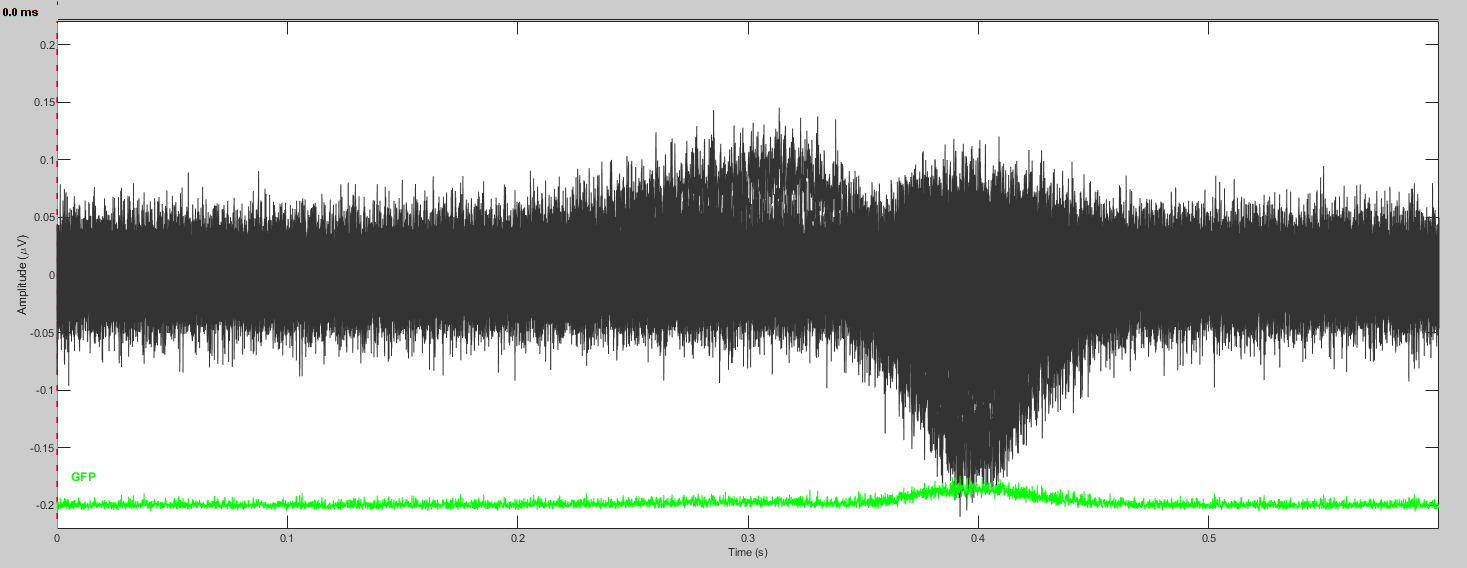
\includegraphics[width=\textwidth]{eeg/eeg-d1n1c9c9.png}
        \caption{Señales de EEG simuladas con BSCR = 20.}
        \label{fig:eeg-d1n1c9c9}
        \vspace{0.5em}
    \end{subfigure}
    \vfill
    \begin{subfigure}{0.9\textwidth}
        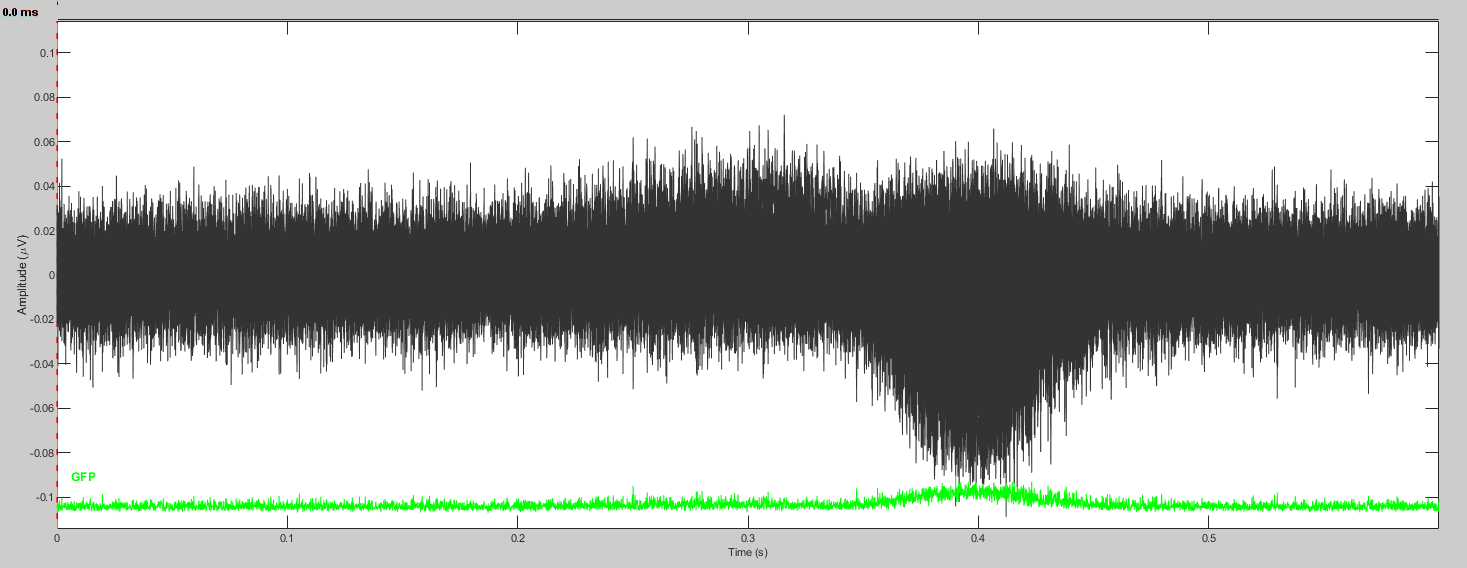
\includegraphics[width=\textwidth]{eeg/eeg-d1n1c10c10.png}
        \caption{Señales de EEG simuladas con BSCR = 80.}
        \label{fig:eeg-d1n1c10c10}
        \vspace{0.5em}
    \end{subfigure}
    \vfill
    \begin{subfigure}{0.9\textwidth}
        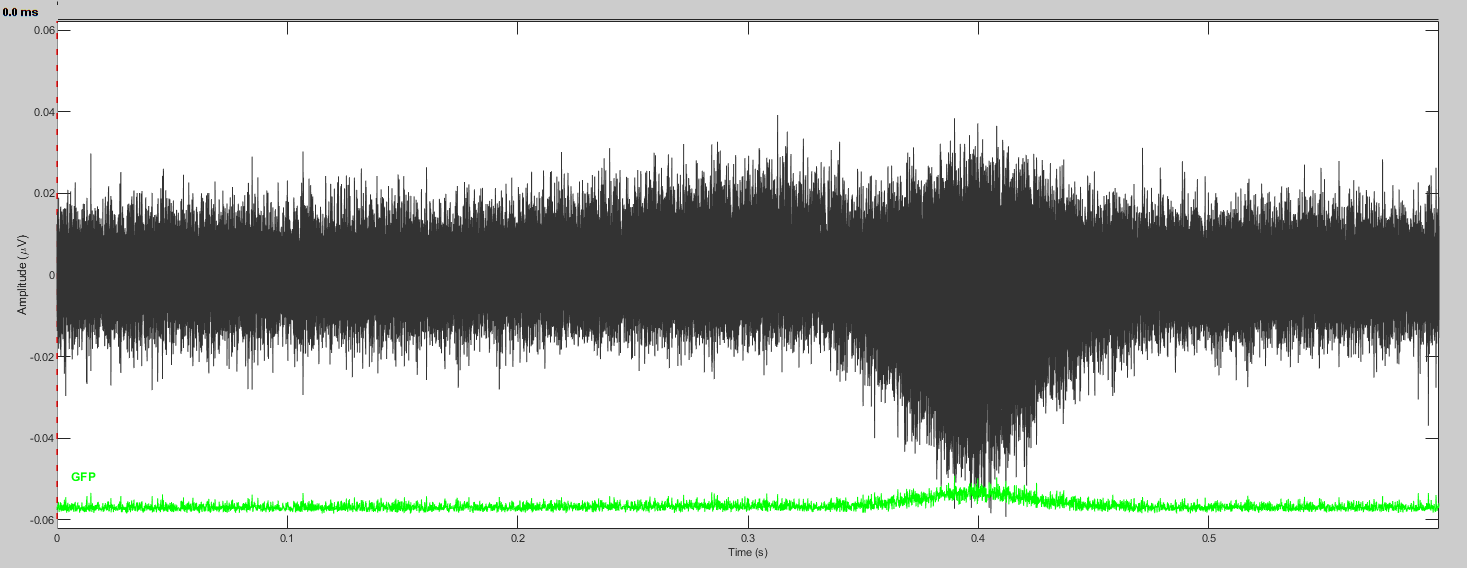
\includegraphics[width=\textwidth]{eeg/eeg-d1n1c2c2.png}
        \caption{Señales de EEG simuladas con BSCR = 200.}
        \label{fig:eeg-d1n1c2c2}
    \end{subfigure}
    \caption{Señales de EEG simuladas con diferentes valores de BSCR.}
    \label{fig:eeg-simulated}
\end{figure}

Observando las señales simuladas, se puede apreciar que a medida que el valor de BSCR disminuye, la amplitud de las señales aumenta. 
Esto no indica que la actividad neuronal sea mayor, sino que la señal es más fácil de detectar por la menor resistencia que presenta al pasar por los tejidos del cráneo.
Cabe mencionar que esta diferencia de amplitud no representa una métrica aceptable para comparar la actividad neuronal entre diferentes valores de BSCR, ya que también influyen otros factores como el ruido introducido en la simulación, el ruido generado por el equipo de medición y en casos reales, las condiciones del paciente.
Independientemente del valor de BSCR, se puede observar que las señales presentan un patrón similar, lo que indica que la actividad neuronal simulada es la misma en todos los casos.

\section{Solución del Problema Inverso}
\label{sec:results:inverse}

En la \cref{fig:inverse-results}, se muestran los resultados de la implementación del problema inverso para el valor de BSCR de 10, 20, 80 y 200 correspondientes al conjunto de señales simuladas con un SNR de 1\% proveniente de la fuente de actividad neuronal ubicada en la zona somatosensorial mencionadas en la \cref{sec:results:direct}.
Dado que las señales de EEG simuladas tienen una componente en el tiempo, el problema inverso se calcula para cada instante de tiempo correspondiente a la frecuencia de muestreo de 1000 Hz, por lo que los resultados mostrados en la \cref{fig:inverse-results} corresponden al instante de tiempo en el que la función del dipolo utilizando como fuente de actividad neuronal se encuentra en su cenit.

\begin{figure}[tbp]
    \centering
    \begin{subfigure}{0.45\textwidth}
        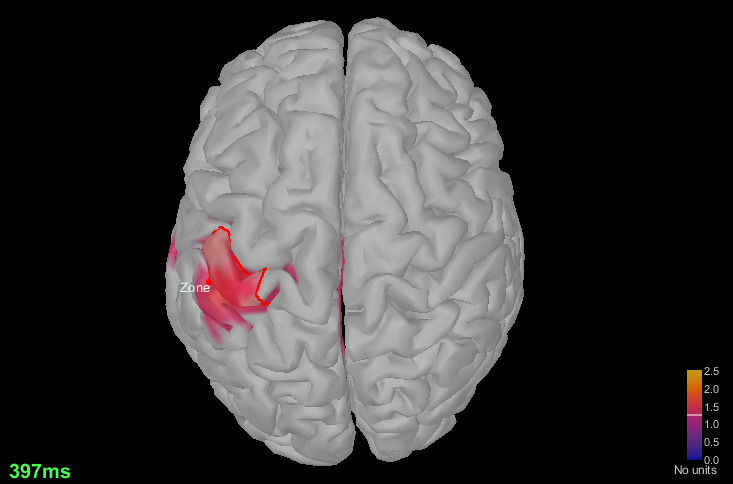
\includegraphics[width=\textwidth]{inverse/inverse-d1n1c2c2.png}
        \caption{PNAI obtenido con BSCR 200 en problema directo e inverso.}
        \label{fig:inverse-d1n1c2c2}
    \end{subfigure}
    \hfill
    \begin{subfigure}{0.45\textwidth}
        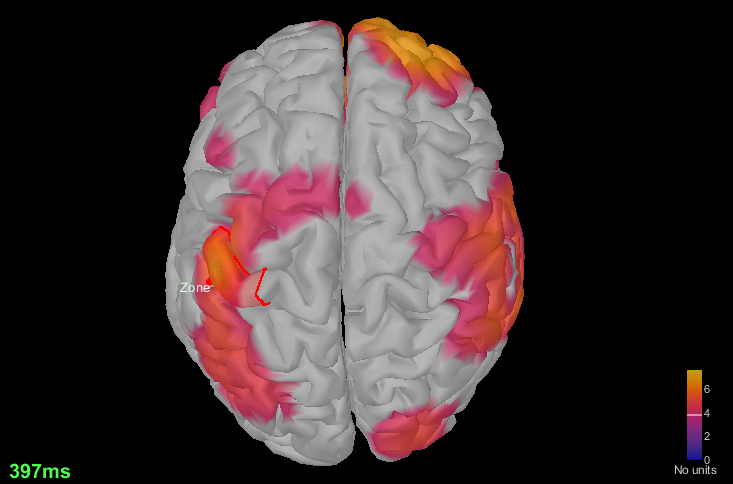
\includegraphics[width=\textwidth]{inverse/inverse-d1n1c8c8.png}
        \caption{PNAI obtenido con BSCR 10 en problema directo e inverso.}
        \label{fig:inverse-d1n2c2c2}
    \end{subfigure}
    \vskip\baselineskip
    \begin{subfigure}{0.45\textwidth}
        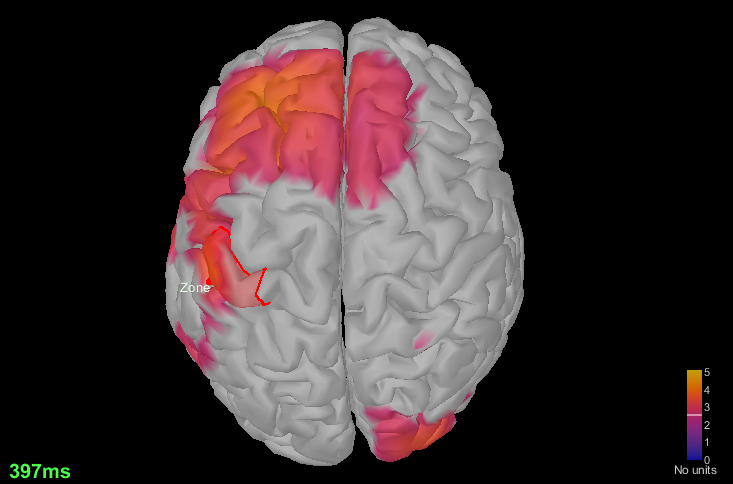
\includegraphics[width=\textwidth]{inverse/inverse-d1n1c9c9.png}
        \caption{PNAI obtenido con BSCR 20 en problema directo e inverso.}
        \label{fig:inverse-d1n3c2c2}
    \end{subfigure}
    \hfill
    \begin{subfigure}{0.45\textwidth}
        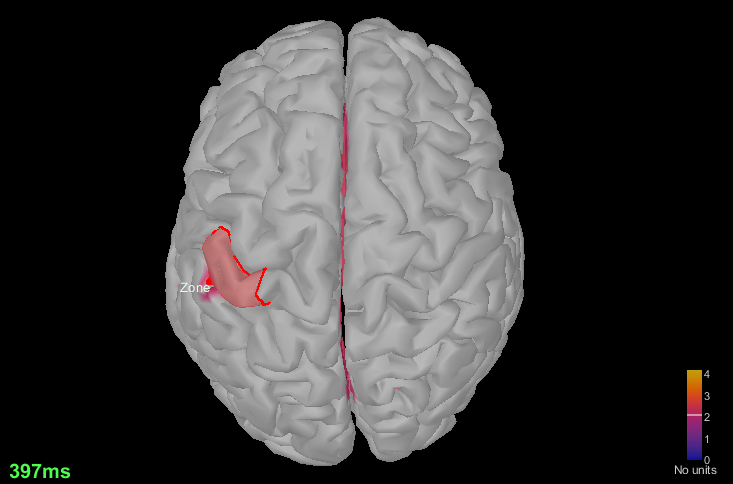
\includegraphics[width=\textwidth]{inverse/inverse-d1n1c10c10.png}
        \caption{PNAI obtenido con BSCR 80 en problema directo e inverso.}
        \label{fig:inverse-d1n4c2c2}
    \end{subfigure}
    \caption{Resultados de la implementación del problema inverso.}
    \label{fig:inverse-results}
\end{figure}


Los resultados mostrados en la figura en cuestión, corresponden a la localización de la fuente de actividad neuronal utilizando el mismo valor de BSCR como parámetro del filtro espacial en la solución del problema inverso y en la simulación de las señales de EEG en el problema directo.
Por lo tanto, se espera que el punto de máxima actividad neuronal proyectado sobre la malla representativa de la corteza cerebral se localice en la misma región y vértice que el dipolo utilizado como fuente de actividad neuronal en la simulación de las señales de EEG.
Justo como en los resultados de la \cref{sec:results:direct}, en la \cref{fig:inverse-results} se aprecia una diferencia en la magnitud del PNAI obtenido, donde a medida que el valor de BSCR disminuye, no solo la magnitud del PNAI aumenta, sino que también el área sobre la que se propaga la actividad neuronal simulada se expande.

\section{Estimación del Error en la Localización de la Fuente de Actividad Neuronal}
\label{sec:results:error}

La estimación del error en la localización se obtuvo con el método descrito en la \cref{sec:methodology:estimator}, mientras que el análisis estadístico del desempeño del estimador se realizó con el método descrito en la \cref{sec:methodology:cbr-analysis}.
Por lo tanto, los resultados presentados corresponden a la diferencia entre la localización de la fuente de actividad neuronal obtenida en el problema inverso y la localización de la fuente de actividad neuronal utilizada en la simulación de las señales de EEG en el problema directo dividida por la distancia media entre los vértices de la malla representativa de la corteza cerebral. 
Para que los resultados obtenidos pudieran ser comparados y representados de manera gráfica, se agruparon los valores del error en la localización de la fuente de actividad neuronal obtenidos en las 100 pruebas de cada permutación de BSCR, SNR y fuente de actividad neuronal.
Se calculó el promedio y la desviación estándar de los valores obtenidos en cada permutación y se presentaron en gráficas de barras de error con la CRB como referencia en el eje horizontal.

\subsection{Error en el grupo de señales de EEG simuladas con el dipolo en la zona somatosensorial y SNR 1\%}
\label{sec:results:error:d1n1}

En la \cref{fig:error-results-d1n1}, se presentan los resultados obtenidos en la estimación del error en la localización de la fuente de actividad neuronal con el dipolo ubicado en la zona somatosensorial (dipolo 1 de acuerdo a nuestro sistema de identificación) y un SNR de 1\%.

Tomando en cuenta los resultados obtenidos y la atipicidad de los valores de BSCR 10 y 200, nos enfocamos en los valores de BSCR 20 y 80, los cuales son los más cercanos a los valores reportados en la literatura y siguen siendo distantes entre sí. 

\begin{figure}[htb]
    \centering
    \begin{subfigure}{0.49\textwidth}
        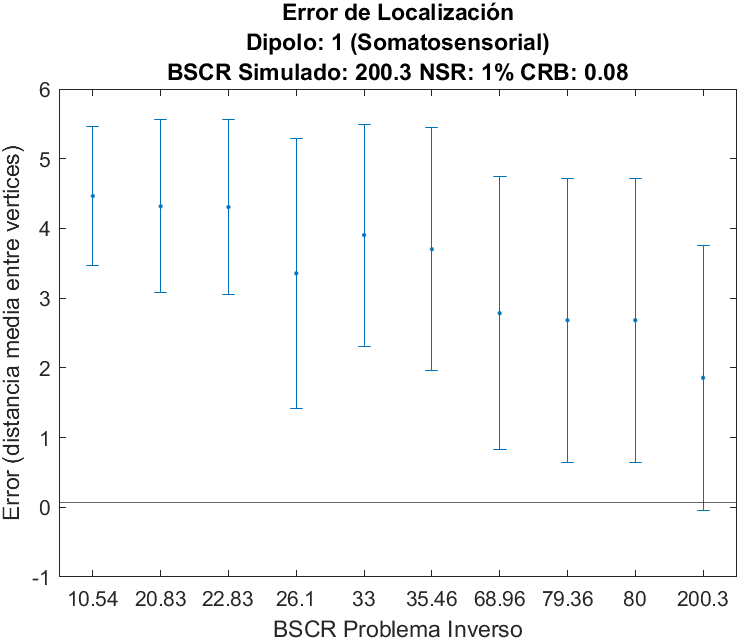
\includegraphics[width=\textwidth]{individual_graphs/d1c2n1.png}
        \caption{Error en la localización de la fuente de actividad neuronal con BSCR 200.3.}
        \label{fig:error-d1c2n1}
    \end{subfigure}
    \hfill
    \begin{subfigure}{0.49\textwidth}
        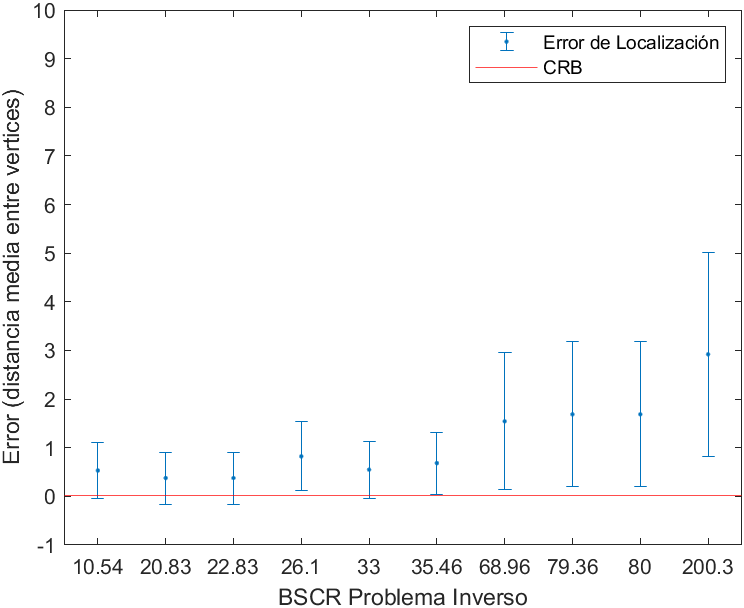
\includegraphics[width=\textwidth]{individual_graphs/d1c8n1.png}
        \caption{Error en la localización de la fuente de actividad neuronal con BSCR 10.54.}
        \label{fig:error-d1c8n1}
    \end{subfigure}
    \vskip\baselineskip
    \begin{subfigure}{0.49\textwidth}
        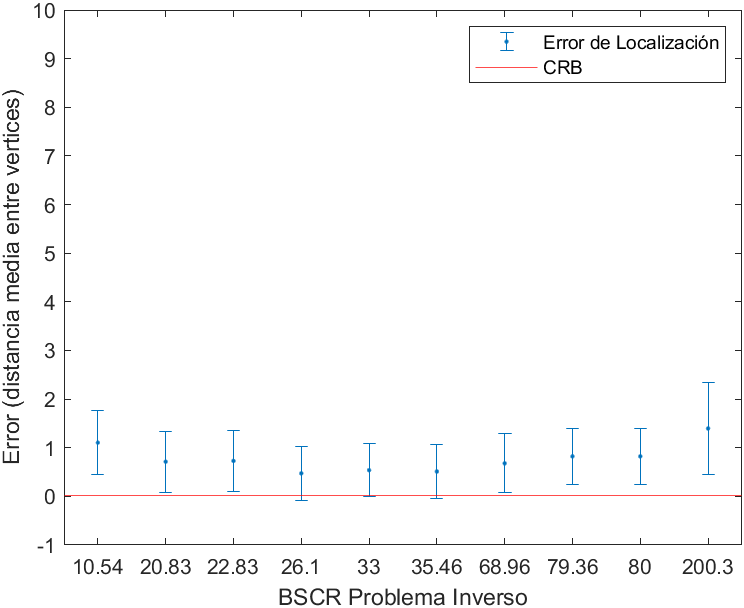
\includegraphics[width=\textwidth]{individual_graphs/d1c9n1.png}
        \caption{Error en la localización de la fuente de actividad neuronal con BSCR 20.83.}
        \label{fig:error-d1c9n1}
    \end{subfigure}
    \hfill
    \begin{subfigure}{0.49\textwidth}
        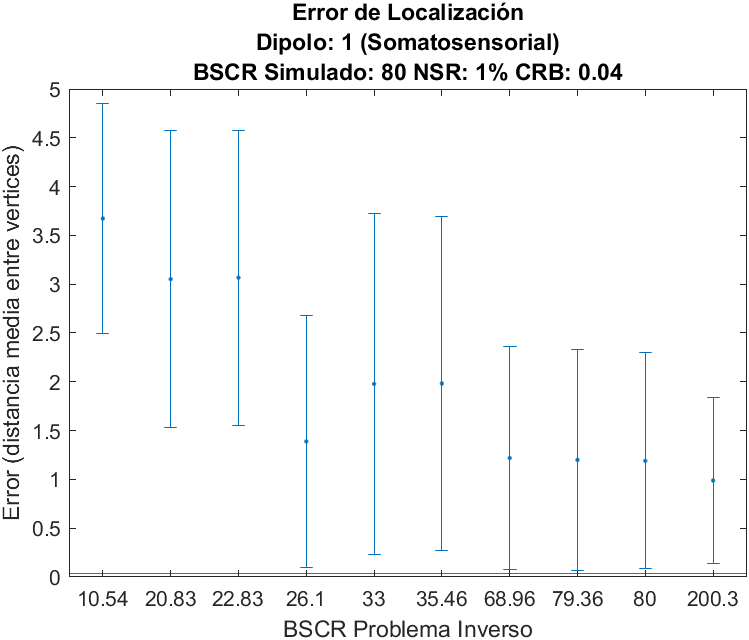
\includegraphics[width=\textwidth]{individual_graphs/d1c10n1.png}
        \caption{Error en la localización de la fuente de actividad neuronal con BSCR 80.}
        \label{fig:error-d1c10n1}
    \end{subfigure}
    \caption{Error incurrido en la localización de la fuente de actividad neuronal en con el dipolo en la zona somatosensorial y SNR 1\%.}
    \label{fig:error-results-d1n1}
\end{figure}

\subsection{Error en el grupo de señales de EEG simuladas en diferentes zonas de la corteza cerebral y niveles de SNR para BSCR = 20 y 80}
\label{sec:results:error:dn-rest}

Con el fin de ampliar el panorama de los datos obtenidos, se presentan los resultados de la estimación del error en la localización de la fuente de actividad neuronal para los valores de BSCR 20 y BSCR 80.
Específicamente, se comparan los resultados obtenidos de la implementación del problema inverso sobre las señales de EEG simuladas con el dipolo ubicado en las zonas auditiva (dipolo 2) y visual (dipolo 3) y con niveles de SNR: 1\%, 5\% y 10\%.

\begin{figure}[hp]
    \centering
    \begin{subfigure}{0.49\textwidth}
        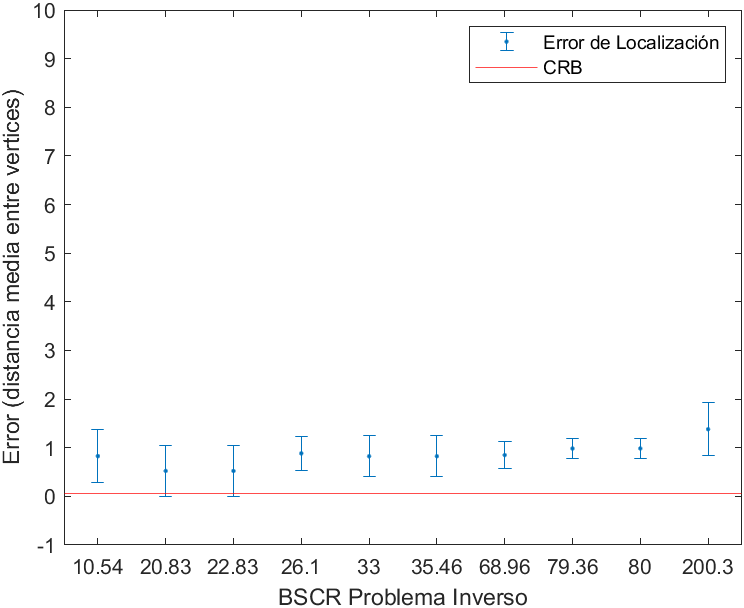
\includegraphics[width=\textwidth]{individual_graphs/d2c9n1.png}
        \caption{Error en la localización de la fuente de actividad neuronal con BSCR 20 y SNR 1\%.}
        \label{fig:error-d2c9n1}
    \end{subfigure}
    \hfill
    \begin{subfigure}{0.49\textwidth}
        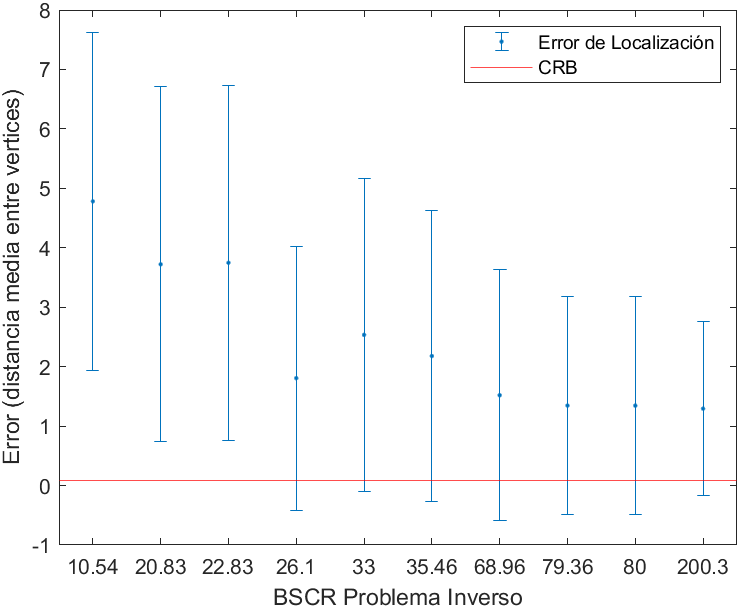
\includegraphics[width=\textwidth]{individual_graphs/d2c10n1.png}
        \caption{Error en la localización de la fuente de actividad neuronal con BSCR 80 y SNR 1\%.}
        \label{fig:error-d2c10n1}
    \end{subfigure}
    \vskip\baselineskip
    \begin{subfigure}{0.49\textwidth}
        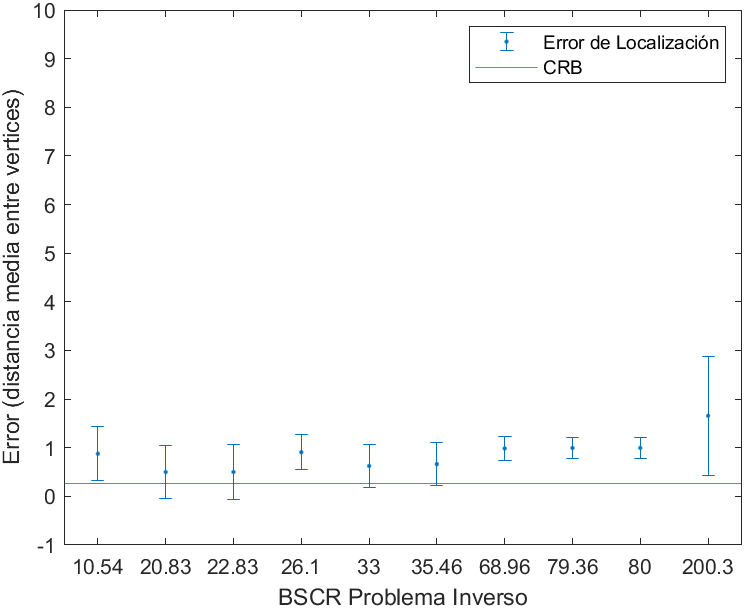
\includegraphics[width=\textwidth]{individual_graphs/d2c9n2.png}
        \caption{Error en la localización de la fuente de actividad neuronal con BSCR 20 SNR 5\%.}
        \label{fig:error-d2c9n2}
    \end{subfigure}
    \hfill
    \begin{subfigure}{0.49\textwidth}
        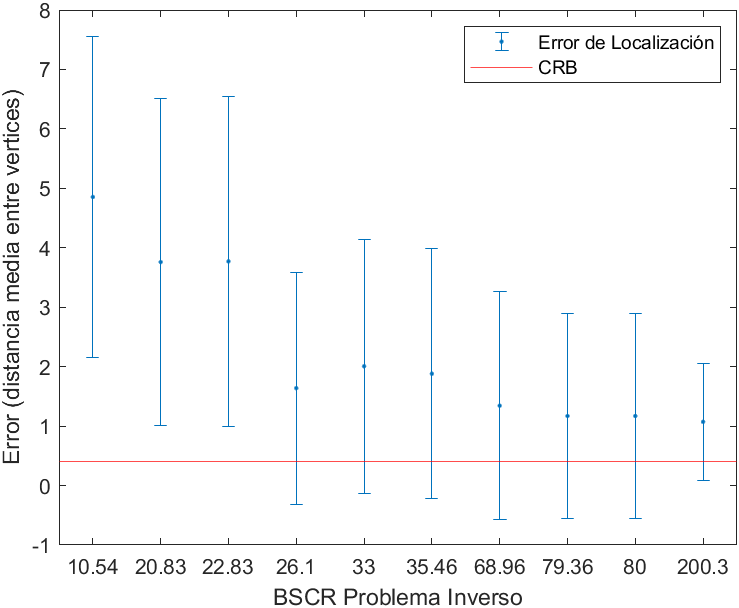
\includegraphics[width=\textwidth]{individual_graphs/d2c10n2.png}
        \caption{Error en la localización de la fuente de actividad neuronal con BSCR 80 y SNR 5\%.}
        \label{fig:error-d2c10n2}
    \end{subfigure}
    \vskip\baselineskip
    \begin{subfigure}{0.49\textwidth}
        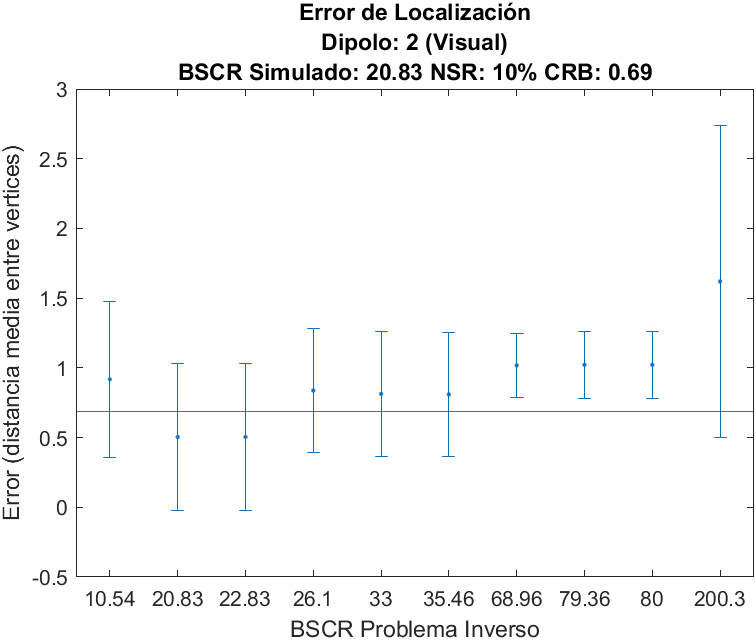
\includegraphics[width=\textwidth]{individual_graphs/d2c9n3.png}
        \caption{Error en la localización de la fuente de actividad neuronal con BSCR 20 y SNR 10\%.}
        \label{fig:error-d2c9n3}
    \end{subfigure}
    \hfill
    \begin{subfigure}{0.49\textwidth}
        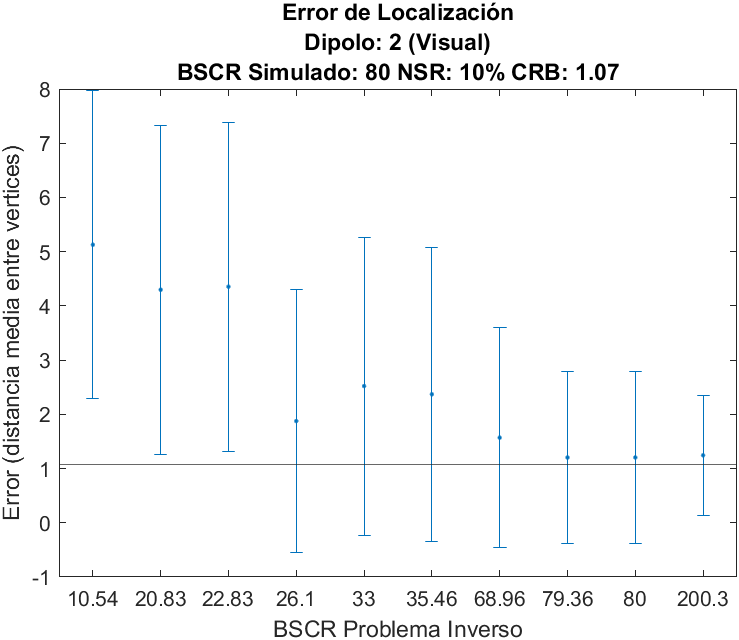
\includegraphics[width=\textwidth]{individual_graphs/d2c10n3.png}
        \caption{Error en la localización de la fuente de actividad neuronal con BSCR 80 y SNR 10\%.}
        \label{fig:error-d2c10n3}
    \end{subfigure}
    \caption{Error incurrido en la localización de la fuente de actividad neuronal en con el dipolo en la zona auditiva y los tres niveles de SNR.}
    \label{fig:error-results-d2}
\end{figure}

En la \cref{fig:error-results-d2}, se aprecia el mismo fenómeno observado en la \cref{sec:results:error:d1n1}, donde se observa una relación positiva entre el error en la localización de la fuente de actividad neuronal y el valor de BSCR.
En el caso del valor de BSCR 20, el error de localización tiene una variabilidad y diferencia menor en la magnitud del error comparando con el valor de BSCR 80.
Su desempeño es consistente y con una buena exactitud incluso al presentar una mayor magnitud de ruido agregado y utilizar valores atípicos de BSCR en la solución del problema inverso como el BSCR 200.
Por otro lado, el valor de BSCR 80 presenta una mayor variabilidad en los resultados obtenidos, únicamente en el caso en el que se implementan valores cercanos a BSCR 80 en la solución del problema inverso se obtiene un error menor y más consistente en la localización de la fuente de actividad neuronal.
Otra observación importante es que en el caso del error incurrido con el BSCR 80 con nivel de SNR: 10\% (\cref{fig:error-d2c9n3}) este es menor que el que la CRB indica posible para un estimador no sesgado.

Estos fenómenos pueden ser atribuidos a la posición del dipolo en la malla representativa de la corteza cerebral. 
Como se mencionó en la \cref{sec:methodology:direct_solved}, el dipolo 2 se encuentra en la corteza visual primaria colocandolo en la región occipital de la malla.
Con esto en mente, revisando la \cref{fig:methodology:model} se puede observar que la región occipital de la malla es la más alejada de los electrodos, además de una menor concentración de estos en comparación con las posicones de los otros dipolos. 
Lo que implica que el desempeño de la solución del problema inverso con el método de elementos de frontera sea menos preciso en la localización de la fuente de actividad neuronal debido a las limitaciones de la técnica.
Quizá una solución a este problema sería utilizar un método de solución más adecuado para este escenario, como el método de elementos finitos, que permite trabajar con potenciales propagados en volumenes anisotrópicos en lugar de una superficies isotrópicas como lo hace el método de elementos de frontera.


\begin{figure}[hp]
    \centering
    \begin{subfigure}{0.49\textwidth}
        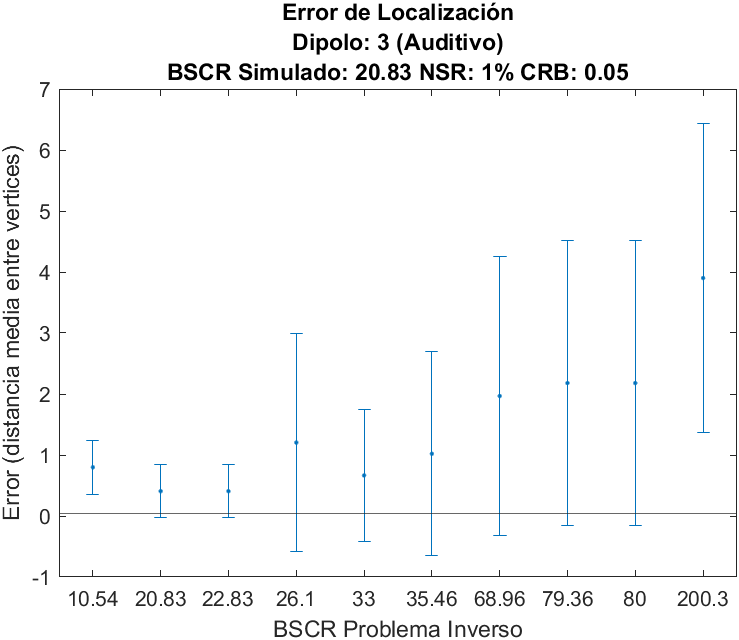
\includegraphics[width=\textwidth]{individual_graphs/d3c9n1.png}
        \caption{Error en la localización de la fuente de actividad neuronal con BSCR 20 y SNR 1\%.}
        \label{fig:error-d3c9n1}
    \end{subfigure}
    \hfill
    \begin{subfigure}{0.49\textwidth}
        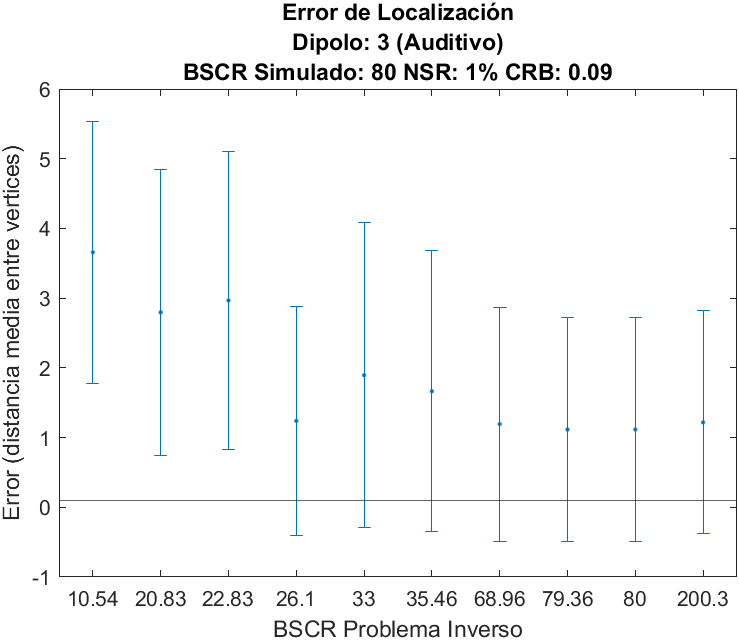
\includegraphics[width=\textwidth]{individual_graphs/d3c10n1.png}
        \caption{Error en la localización de la fuente de actividad neuronal con BSCR 80 y SNR 1\%.}
        \label{fig:error-d3c10n1}
    \end{subfigure}
    \vskip\baselineskip
    \begin{subfigure}{0.49\textwidth}
        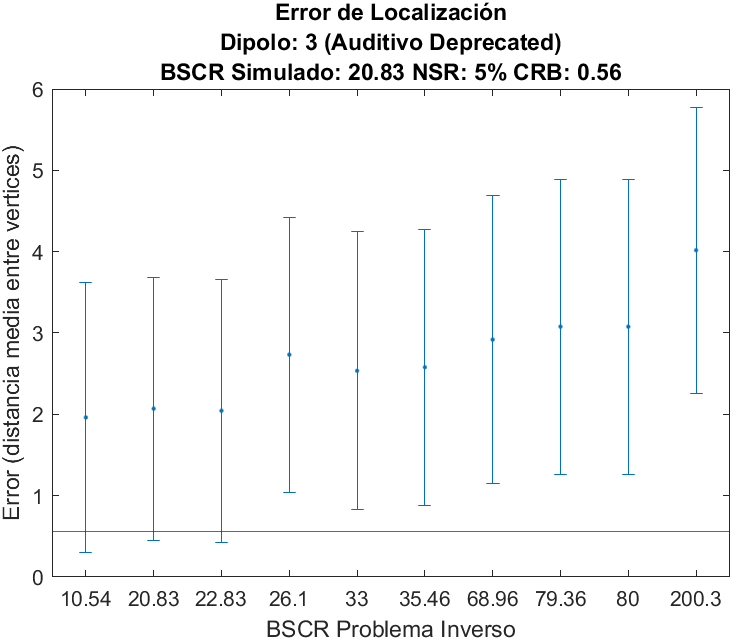
\includegraphics[width=\textwidth]{individual_graphs/d3c9n2.png}
        \caption{Error en la localización de la fuente de actividad neuronal con BSCR 20 SNR 5\%.}
        \label{fig:error-d3c9n2}
    \end{subfigure}
    \hfill
    \begin{subfigure}{0.49\textwidth}
        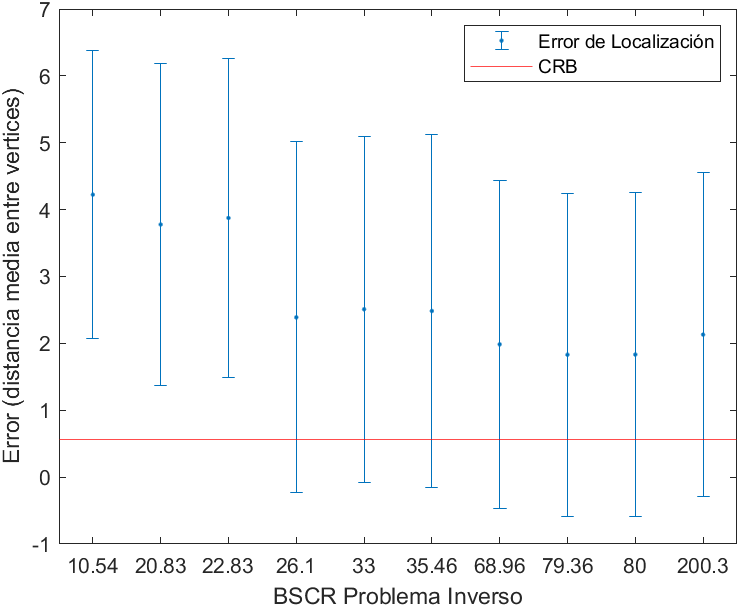
\includegraphics[width=\textwidth]{individual_graphs/d3c10n2.png}
        \caption{Error en la localización de la fuente de actividad neuronal con BSCR 80 y SNR 5\%.}
        \label{fig:error-d3c10n2}
    \end{subfigure}
    \vskip\baselineskip
    \begin{subfigure}{0.49\textwidth}
        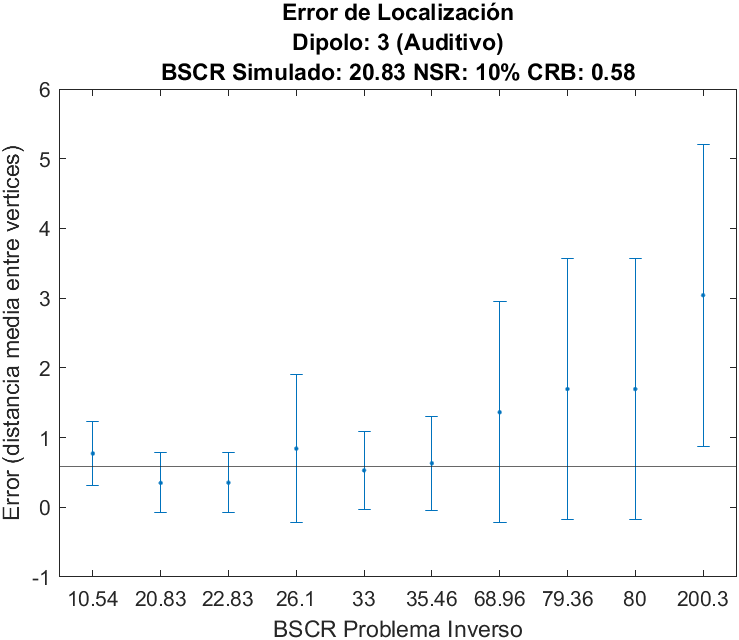
\includegraphics[width=\textwidth]{individual_graphs/d3c9n3.png}
        \caption{Error en la localización de la fuente de actividad neuronal con BSCR 20 y SNR 10\%.}
        \label{fig:error-d3c9n3}
    \end{subfigure}
    \hfill
    \begin{subfigure}{0.49\textwidth}
        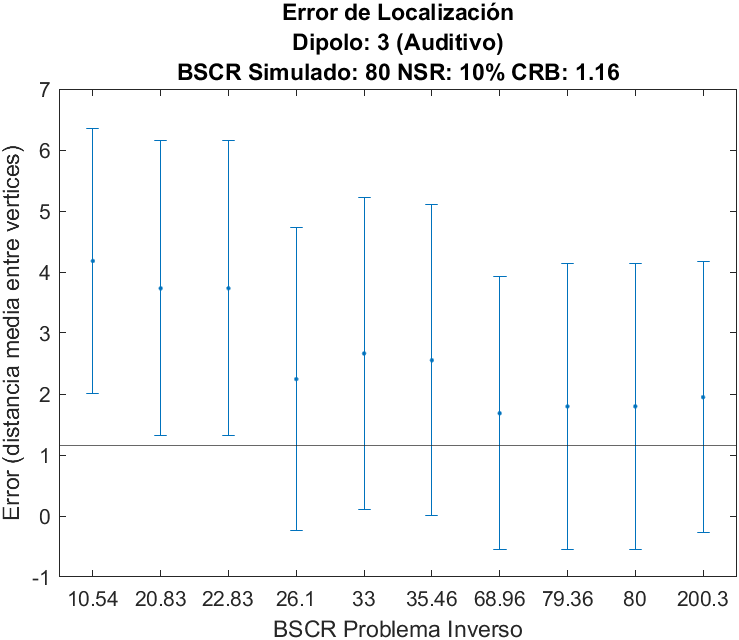
\includegraphics[width=\textwidth]{individual_graphs/d3c10n3.png}
        \caption{Error en la localización de la fuente de actividad neuronal con BSCR 80 y SNR 10\%.}
        \label{fig:error-d3c10n3}
    \end{subfigure}
    \caption{Error incurrido en la localización de la fuente de actividad neuronal en con el dipolo en la zona auditiva y los tres niveles de SNR.}
    \label{fig:error-results-d3}
\end{figure}

En el caso del dipolo 3, ubicado en la corteza auditiva primaria, se observa un patrón similar al de los resultados anteriores, teniendo el BSCR 20 un mejor desempeño en la localización de la fuente de actividad neuronal y una menor variabilidad en los resultados obtenidos.
También se presenta el mismo fenómeno observado que en las pruebas con el dipolo 2, donde el error incurrido con el BSCR 80 y SNR 10\% es menor que el que la CRB indica posible para un estimador no sesgado.
Siendo nuestra intención probar casos distintos, el dipolo 3 fue colocado en uno de los pliegues de la corteza auditiva primaria, haciendo la dirección del campo eléctrico generado por el dipolo paralelo al resto de las mallas que componen la cabeza.
dipolo perpendicular al resto de las mallas que componen la cabeza.
Esta posición del dipolo le da la particularidad de encontraste en una región de la malla con una mayor concentración de vértices, lo que implica que la solución del problema inverso con el método de elementos de frontera sea más precisa en la localización de la fuente de actividad neuronal por el mayor número de puntos de referencia en la malla a comparación de otras zonas, lo que representa que en efecto en este caso es un estimador sesgado. \TODO{esto es un sesgo?}

\section{Desempeño del Uso de Diferentes Valores de BSCR en la Simulación y Localización de Fuentes de Actividad Neuronal}
\label{sec:results:bscr-performance}

\begin{figure}[htbp]
    \centering
    \begin{subfigure}{0.49\textwidth}
        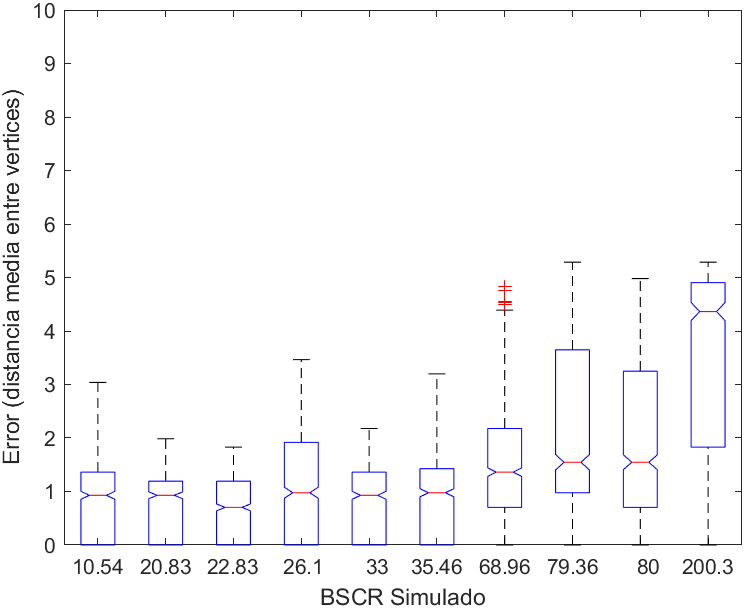
\includegraphics[width=\textwidth]{overall_bscr_error_boxplots_percentile/d1n1.png}
        \caption{Error en la localización de la fuente de actividad neuronal de diferentes BSCR: Dipolo 1, SNR 1\%.}
        \label{fig:error-overall-d1n1}
    \end{subfigure}
    \hfill
    \begin{subfigure}{0.49\textwidth}
        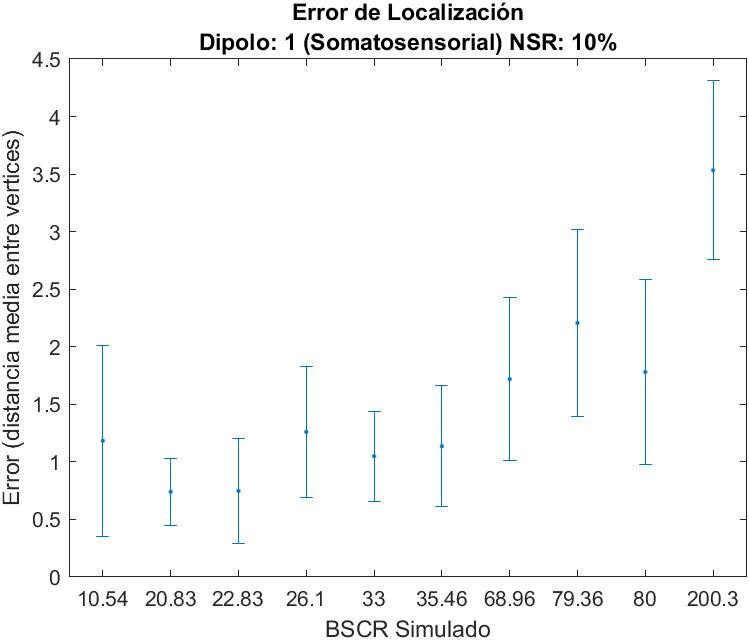
\includegraphics[width=\textwidth]{overall_bscr_error_boxplots_percentile/d1n3.png}
        \caption{Error en la localización de la fuente de actividad neuronal de diferentes BSCR: Dipolo 1, SNR 10\%.}
        \label{fig:crb-overall-d1n3}
    \end{subfigure}
    \vskip\baselineskip
    \begin{subfigure}{0.49\textwidth}
        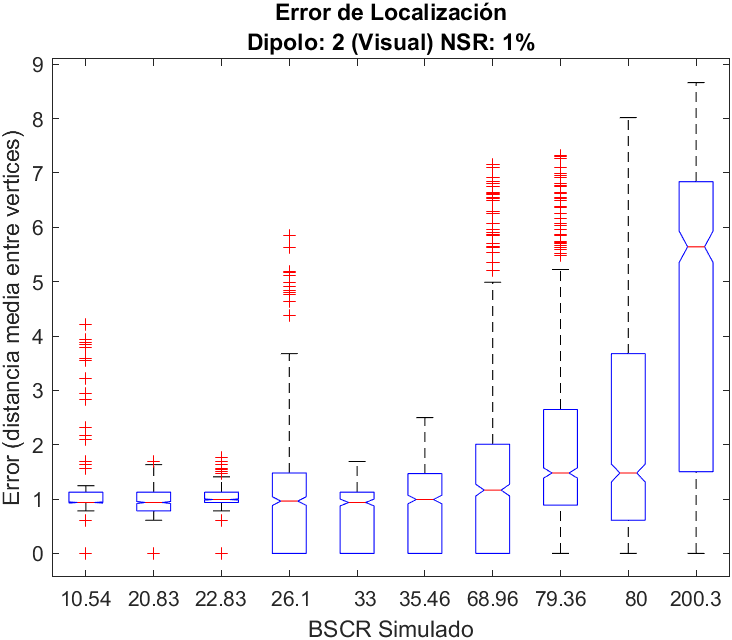
\includegraphics[width=\textwidth]{overall_bscr_error_boxplots_percentile/d2n1.png}
        \caption{Error en la localización de la fuente de actividad neuronal de diferentes BSCR: Dipolo 2, SNR 1\%.}
        \label{fig:error-overall-d2n1}
    \end{subfigure}
    \hfill
    \begin{subfigure}{0.49\textwidth}
        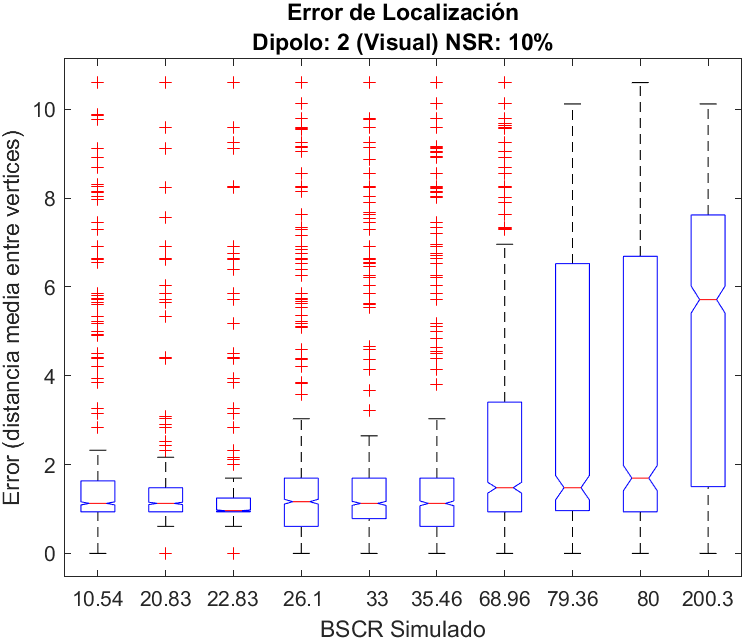
\includegraphics[width=\textwidth]{overall_bscr_error_boxplots_percentile/d2n3.png}
        \caption{Error en la localización de la fuente de actividad neuronal de diferentes BSCR: Dipolo 2, SNR 10\%.}
        \label{fig:crb-overall-d2n3}
    \end{subfigure}
    \vskip\baselineskip
    \begin{subfigure}{0.49\textwidth}
        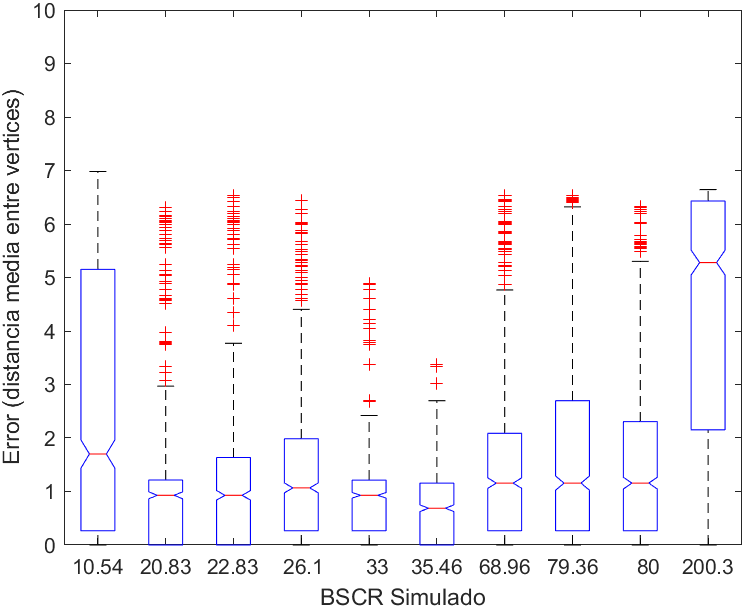
\includegraphics[width=\textwidth]{overall_bscr_error_boxplots_percentile/d3n1.png}
        \caption{Error en la localización de la fuente de actividad neuronal de diferentes BSCR: Dipolo 3, SNR 1\%.}
        \label{fig:error-overall-d3n1}
    \end{subfigure}
    \hfill
    \begin{subfigure}{0.49\textwidth}
        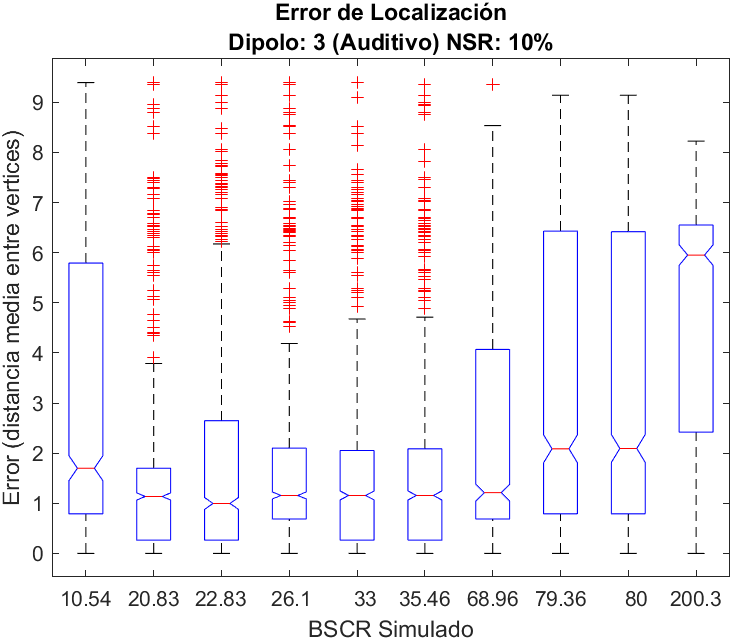
\includegraphics[width=\textwidth]{overall_bscr_error_boxplots_percentile/d3n3.png}
        \caption{Error en la localización de la fuente de actividad neuronal de diferentes BSCR: Dipolo 3, SNR 10\%.}
        \label{fig:crb-overall-d3n3}
    \end{subfigure}
    \caption{Desempeño del uso de diferentes valores de BSCR en la simulación y localización de fuentes de actividad neuronal.}
    \label{fig:bscr-performance}
\end{figure}

En la \cref{fig:bscr-performance}, se presentan los resultados obtenidos en la estimación del error en la localización de la fuente de actividad neuronal para cada uno de los BSCR involucrados en el estudio, agrupados por el dipolo y nivel de ruido correspondiente.
A detalle, el eje horizontal de cada gráfica representa los valores de BSCR utilizados en la simulación de las señales de EEG y el eje vertical representa el error general en la localización de la fuente de actividad neuronal obtenido en las 100 pruebas de cada permutación de BSCR en el problema inverso, por lo tanto, se trata de una matriz de 1000$\times$10.
Se eligió mostrar los resultados del nivel de SNR 1\% y 10\% para cada dipolo, ya que estos representan los extremos en la relación señal-ruido y permiten observar el desempeño del estimador en condiciones de ruido bajo y ruido alto.

En general, se observa que los valores de BSCR en un rango de 20-35 presentan un mejor desempeño en la localización de la fuente de actividad neuronal, además de una diferencia no significativa en variabilidad en la mayoría de los casos, denotada por la intersección de los intervalos de confianza en las gráficas de caja.
Esto es un indicativo de que los valores de BSCR en este rango pueden ser utilizados en la solución del problema inverso con diferentes pacientes y condiciones de ruido, sin afectar significativamente la precisión en la localización de la fuente de actividad neuronal.

Este resultado es relevante, ya que permite a los investigadores y médicos utilizar un rango de valores de BSCR en la localización de fuentes de actividad neuronal sin afectar la exactitud del diagnóstico por la variación en la conductividad de los tejidos del cráneo, ya sean por diferencias en la edad, género, enfermedades o condiciones del paciente.

